\subsection{Belysningsmodell}

\begin{frame}
\frametitle{Belysningsmodell}

\begin{columns}[c]

\column{.5\textwidth}

\begin{itemize}[<+(2)->]
\item Fysikaliskt härledd
\item Utgår ifrån renderingsekvationen
\item Statistisk modell (använder vågspektrumet)
\item Snarlik i utseendet till Blinn--Phong
\end{itemize}

\column{.5\textwidth}

\uncover<2->{
\begin{figure}
\centering
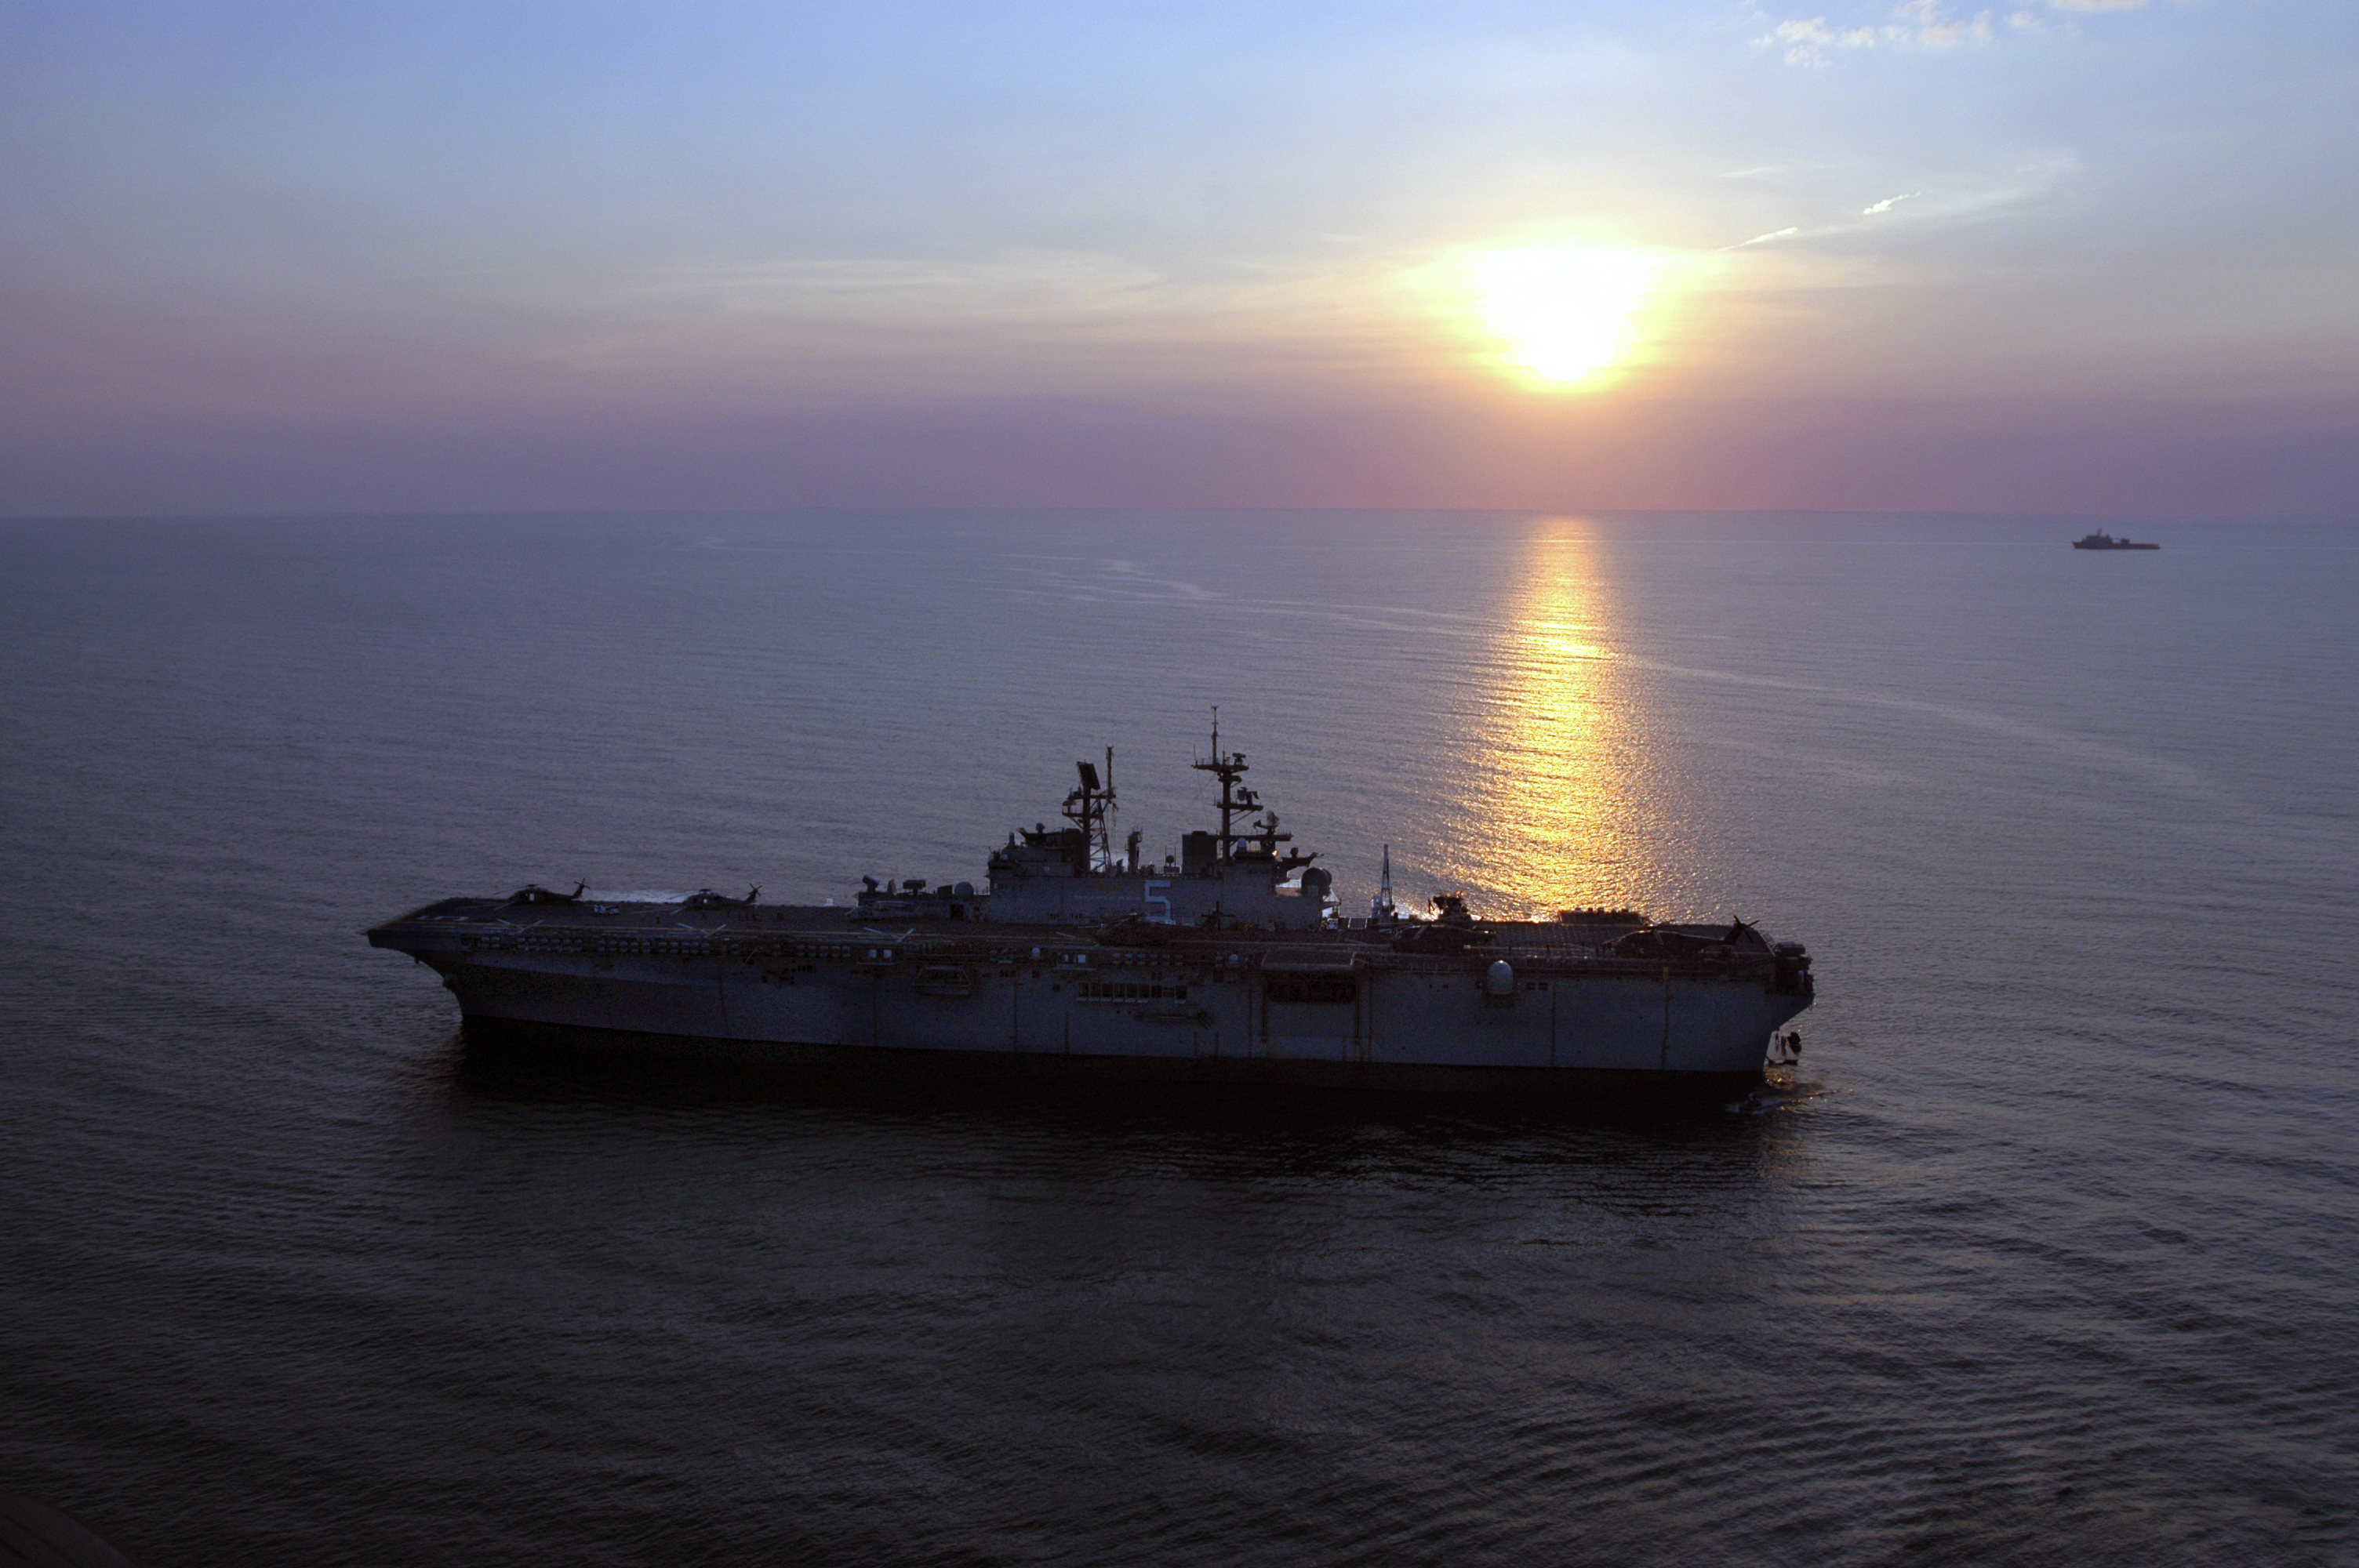
\includegraphics[width=\textwidth]{../Report/Images/Public_domain/Sunglint_close_to_the_horizon}
\end{figure}
}

\end{columns}

\end{frame}
